\documentclass[12pt, letterpaper]{article}
\usepackage[utf8]{inputenc}
\usepackage{amsmath}
\usepackage{graphicx}
\graphicspath{ {.} }
\usepackage{wrapfig}
 
\title{Math 789 Assignment 3}
\author{Brendan Drachler}
\date{\today}

\begin{document}

\begin{titlepage}
\maketitle
\end{titlepage}
\section*{Bishop 2.1}
Beginning from Eq. 2.1, 
\begin{equation}
P(x) = \frac{1}{{\sigma \sqrt {2\pi } }}e^{{{ - \left( {x - \mu } \right)^2 } \mathord{\left/ {\vphantom {{ - \left( {x - \mu } \right)^2 } {2\sigma ^2 }}} \right. \kern-\nulldelimiterspace} {2\sigma ^2 }}}
\end{equation}
We want to use the fact that:
\begin{equation}
\int_{-\infty}^{\infty} e^{\frac{\lambda}{2} x^2} dx = (\frac{2 \pi}{\lambda})^{\frac{1}{2}}
\end{equation}
To verify Eq. 2.2 and 2.3 as well as to prove that $\int p(x) dx = 1$. I'll start by proving the latter.


By defining $\lambda = \frac{1}{\sigma^2}$ and integrating Eq. 1, we can rewrite it as, 

\begin{equation}
\int p(x) dx = \int_{-\infty}^{\infty} \frac{1}{{\sigma \sqrt {2\pi } }}e^{\frac{-x^2}{2} \lambda} = (\frac{2 \pi}{\lambda})^{\frac{1}{2}} (\frac{1}{2 \pi})^{\frac{1}{2}} (\frac{1}{\sigma}) 
\end{equation}
\begin{equation}
\downarrow
\end{equation}
\begin{equation}
(\frac{1}{\sigma^2})^{\frac{1}{2}} (\frac{1}{\sigma}) = 1
\end{equation}

Now, to prove Eq. 2.2 in Bishop, we have to solve.

\begin{equation}
\int_{-\infty}^{\infty}  \frac{x}{{\sigma \sqrt {2\pi } }}e^{{{ - \left( {x - \mu } \right)^2 } \mathord{\left/ {\vphantom {{ - \left( {x - \mu } \right)^2 } {2\sigma ^2 }}} \right. \kern-\nulldelimiterspace} {2\sigma ^2 }}} dx
\end{equation}
\begin{equation}
\downarrow
\end{equation}
\begin{equation}
\frac{e^{-(x - \mu )^2/(2 \sigma^2)} + (\frac{\pi}{2})^{\frac{1}{2}} \mu \sigma erf(\frac{x - \mu}{\sqrt{2}\sigma})}{\sqrt{2 \pi} \sigma}\rvert_{-\infty}^{\infty} = \mu
\end{equation}
This validates Eq. 2.2. Now for Eq. 2.3:
\begin{equation}
\int_{-\infty}^{\infty}  \frac{(x - \mu)^2}{{\sigma \sqrt {2\pi } }}e^{{{ - \left( {x - \mu } \right)^2 } \mathord{\left/ {\vphantom {{ - \left( {x - \mu } \right)^2 } {2\sigma ^2 }}} \right. \kern-\nulldelimiterspace} {2\sigma ^2 }}} dx
\end{equation}
\begin{equation}
\downarrow
\end{equation}
\begin{equation}
\frac{1}{2} \sigma (\sigma  erf(\frac{x - \mu}{\sqrt{2}\sigma}) + \sqrt{\frac{2}{\pi}} (\mu - x) e^{-(x - \mu )^2/(2 \sigma^2)}) \rvert_{-\infty}^{\infty} = \frac{1}{2} \sigma (\sigma + \sigma) = \sigma^2
\end{equation}
This validates Eq. 2.3 as well!

\section*{Bishop 2.3}
Starting from Eq. 2.1:
\begin{equation}
P(x) = \frac{1}{{\sigma \sqrt {2\pi } }}e^{{{ - \left( {x - \mu } \right)^2 } \mathord{\left/ {\vphantom {{ - \left( {x - \mu } \right)^2 } {2\sigma ^2 }}} \right. \kern-\nulldelimiterspace} {2\sigma ^2 }}}
\end{equation}
and utilizing
\begin{equation}
E = - \ln L(\theta) = - \sum_{n=1}^{N} \ln P(x^n | \theta)
\end{equation}

Plugging in $P(x)$, we can simplify E to:

\begin{equation}
E = -\frac{N}{2} \ln 2 \pi - \frac{N}{2} \ln \sigma^2 - \frac{1}{2 \sigma^2} \sum_{j-1}^N (x_j - \mu)^2
\end{equation}

We can now differentiate with respect to the two variables, $\mu$ and $\sigma^2$. 

\begin{equation}
\frac{\partial E}{\partial \mu} = \frac{1}{2 \sigma^2} \sum_{j-1}^N 2 (x_j - \mu) = 0 
\end{equation}
\begin{equation}
\sum_{j-1}^N x_j - \sum_{j-1}Nn \mu = 0
\end{equation}
\begin{equation}
\sum_{j-1}^N x_j - N \mu = 0
\end{equation}
\begin{equation}
\frac{1}{N}\sum_{j-1}^N x_j  = \mu
\end{equation}
This reproduces Bishop Eq. 2.21. Now we can differentiate with respect to $\sigma^2$.  
\begin{equation}
\frac{\partial E}{\partial \sigma^2} = -\frac{N}{2 \sigma^2} + \frac{1}{2 \sigma^4} \sum_{j-1}^N (x_j - \mu)^2 = 0 
\end{equation}
Multiplying by $\sigma^2$:
\begin{equation}
\frac{N \sigma^2}{2} - \frac{1}{2} \sum_{j-1}^n (x_j - \mu)^2 = 0 
\end{equation}
\begin{equation}
\sigma^2 = \frac{1}{N} \sum_{j-1}^n (x_j - \mu)^2
\end{equation}
This validates Bishop Eq. 2.22.

\section*{Bishop 2.5}
As usual, we will begin by assuming a distribution given by Bishop Eq. 2.1:
\begin{equation}
p(x^n | \mu) = \frac{1}{{\sigma \sqrt {2\pi } }}e^{{{ - \left( {x - \mu } \right)^2 } \mathord{\left/ {\vphantom {{ - \left( {x - \mu } \right)^2 } {2\sigma ^2 }}} \right. \kern-\nulldelimiterspace} {2\sigma ^2 }}}
\end{equation}
and a prior distribution given by:
\begin{equation}
p_0(\mu) = \frac{1}{{\sigma_o \sqrt {2\pi } }}e^{{{ - \left( {\mu - \mu_o } \right)^2 } \mathord{\left/ {\vphantom {{ - \left( {x - \mu } \right)^2 } {2\sigma_o ^2 }}} \right. \kern-\nulldelimiterspace} {2\sigma_o ^2 }}}
\end{equation}
We know that the product of these two will result in an exponential term and a constant term. My goal is to only analyze what will happen inside the exponential term because if are able to get it in the form $exp(-\frac{1}{2} \frac{\mu - \mu_N}{\sigma_N^2})$, we can deduce what $\mu_N$ and $\sigma_N^2$ are.
Multiplying the two distributions above, calling the catch all constant out front, $A$, and focusing on the $exp()$ term will result in:
\begin{equation}
p_N(\mu | \chi) = A \ exp(- \frac{(\mu - \mu_o)^2}{2 \sigma_o^2} + \sum_{n=1}^N - \frac{(x^n - \mu)^2}{2 \sigma^2})
\end{equation}
Any term not containing a $\mu$ is in essence a multiplicative term that we will wrap up into $A$. With this in mind, we will foil and hide all unnecessary terms. 
\begin{equation}
p_N(\mu | \chi) = A \ exp(-\frac{1}{2} \frac{(\sigma^2 + N \sigma_o^2)\mu^2 - 2 (\sigma^2 \mu_o + N \overline{x} \sigma_o^2) \mu}{\sigma^2 \sigma_o^2})
\end{equation}
We want to get rid of the coefficient in front of the $\mu^2$ term so we can complete the square easily.
\begin{equation}
p_N(\mu | \chi) = A \ exp(-\frac{1}{2} \frac{\mu^2 - 2 \frac{(\sigma^2 \mu_o + N \overline{x} \sigma_o^2)}{(\sigma^2 + N \sigma_o^2)}\mu}{\frac{\sigma^2 \sigma_o^2}{\sigma^2 + N \sigma_o^2}} )
\end{equation}
Completing the square in the numerator leads to:
\begin{equation}
p_N(\mu | \chi) = A \ exp(-\frac{1}{2} \frac{(\mu - \frac{N \overline{x} \sigma_o^2 + \sigma^2 \mu_o}{\sigma^2 + N \sigma_o^2})^2}{\frac{\sigma_o^2 \sigma^2}{\sigma^2 + N \sigma_o^2}})
\end{equation}
We finally have this in the form we need!
The term subtracted from the $\mu$ is $\mu_N$ and the term in the denominator is $\sigma_N^2$.
\begin{equation}
\mu_N = \frac{N \overline{x} \sigma_o^2 + \sigma^2 \mu_o}{\sigma^2 + N \sigma_o^2} \ , \ \sigma_N^2 = \frac{\sigma_o^2 \sigma^2}{\sigma^2 + N \sigma_o^2}
\end{equation}

\section*{Bishop 2.9}
I've generated two multivariate samples with the covariance matrix equal to the identity and the mean of each sample being, $\mu_1 = 10$ and $\mu_2 = 5$. 

My K-nearest neighbor predictor for different values of K are below. The $k=1$ case seems to be overfitting severely. It is making an effort to separate every point. It likely could not be generalized.  


\begin{figure}[h]
\caption{KNN best fit with k = 1.}
\centering
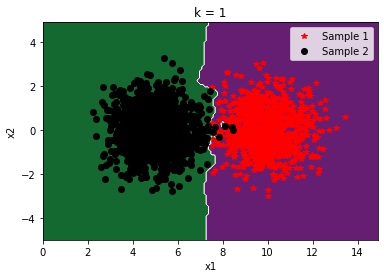
\includegraphics[width=0.5\linewidth]{KNN_1.png}
\end{figure}

The $k=5$ case does a good job of separating the two populations with good generality.

\begin{figure}[h]
\caption{KNN best fit with k = 5.}
\centering
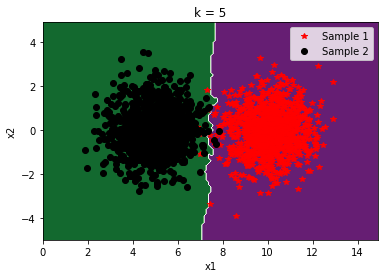
\includegraphics[width=0.5\linewidth]{KNN_5.png}
\end{figure}

The $k=20$ case seems to be averaging the populations which is arguably not the best fit. 

\begin{figure}[h]
\caption{KNN best fit with k = 20.}
\centering
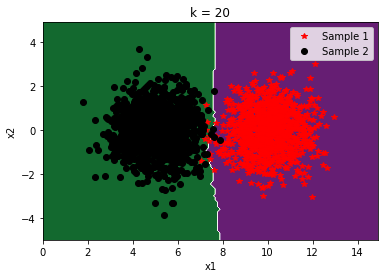
\includegraphics[width=0.5\linewidth]{KNN_20.png}
\end{figure}

\section*{Bishop 2.10}
\begin{figure}[h]
\caption{Verifies the inequality $\ln x \leq \ x-1$}
\centering
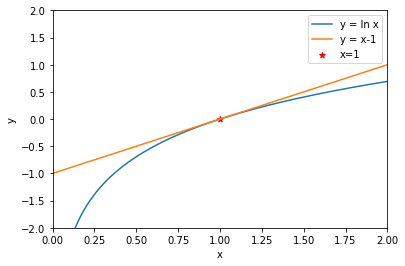
\includegraphics[width=0.8\linewidth]{Kullback_Leibler.png}
\end{figure}

Now, we will maximize $\ln x - \ x-1$.The inequality says this should always be negative expect at $x=1$. Therefore, we expect the maximum to be at $x=1$. 

\begin{equation}
\frac{d}{dx}( \ln x - \ x-1) = 0
\end{equation}
\begin{equation}
\frac{1}{x} - 1 = 0
\end{equation}
\begin{equation}
x = 1
\end{equation}

Now, we will analyze the Kullback-Leibler distance is given by:
\begin{equation}
L = - \int p(x) \ln \frac{\tilde{p}(x)}{p(x)} dx
\end{equation}
We will draw a parallel with the first part of this exercise by saying $\frac{\tilde{p}(x)}{p(x)} = x$. 

\begin{equation}
\int p(x) \ln \frac{\tilde{p}(x)}{p(x)} dx \leq \int p(x) (\frac{\tilde{p}(x)}{p(x)}-1) dx 
\end{equation}

Differentiating both sides leads to:

\begin{equation}
 \ln \frac{\tilde{p}(x)}{p(x)} \leq (\frac{\tilde{p}(x)}{p(x)}-1)  
\end{equation}

\begin{equation}
 \ln \frac{\tilde{p}(x)}{p(x)} - (\frac{\tilde{p}(x)}{p(x)}-1)  \leq 0
\end{equation}

Find the maximum, which is identical to what was done above:

\begin{equation}
\tilde{p}(x) = p(x)
\end{equation}

Therefore, $L \geq 0$ with equality if $\tilde{p}(x) = p(x)$.

\section*{Bishop 2.11}
Applying the Lagrangian to this case with the constraint, $\sum_i q_i = 1$. 

\begin{equation}
- \sum_i p_i \ln (\frac{q_i}{p_i}) + \lambda (\sum_i q_i - 1) = 0
\end{equation}

\begin{equation}
- \sum_i p_i \ln(q_i) + \sum_i p_i \ln(p_i) + \lambda \sum_i q_i - \lambda = 0 (p_i + q_i + \lambda)
\end{equation}

Now, I will use a undetermined coefficients type method to solve this.

\begin{equation}
\lambda \sum_i q_i - \lambda = 0
\end{equation}
\begin{equation}
\sum_i q_i = 1
\end{equation}

This proves our constraint. Now to prove the second part, 

\begin{equation}
-\ln (q_i) + \ln (p_i) = 0
\end{equation}
\begin{equation}
q_i = p_i
\end{equation}

We've shown in the previous problem that if two discrete distributions are equal, the Kullback-Leibler distance is 0. And in this problem we proved that $p_i = q_i$. Therefore, the KL distance between them is 0.

\end{document}